\section{Specific requirements}

\subsection{External Interface Requirements}
In this section are described details about user interfaces, hardware and application programming interfaces.

\subsubsection{User Interfaces}
\begin{figure}[H]
    \subfloat[Details]{
        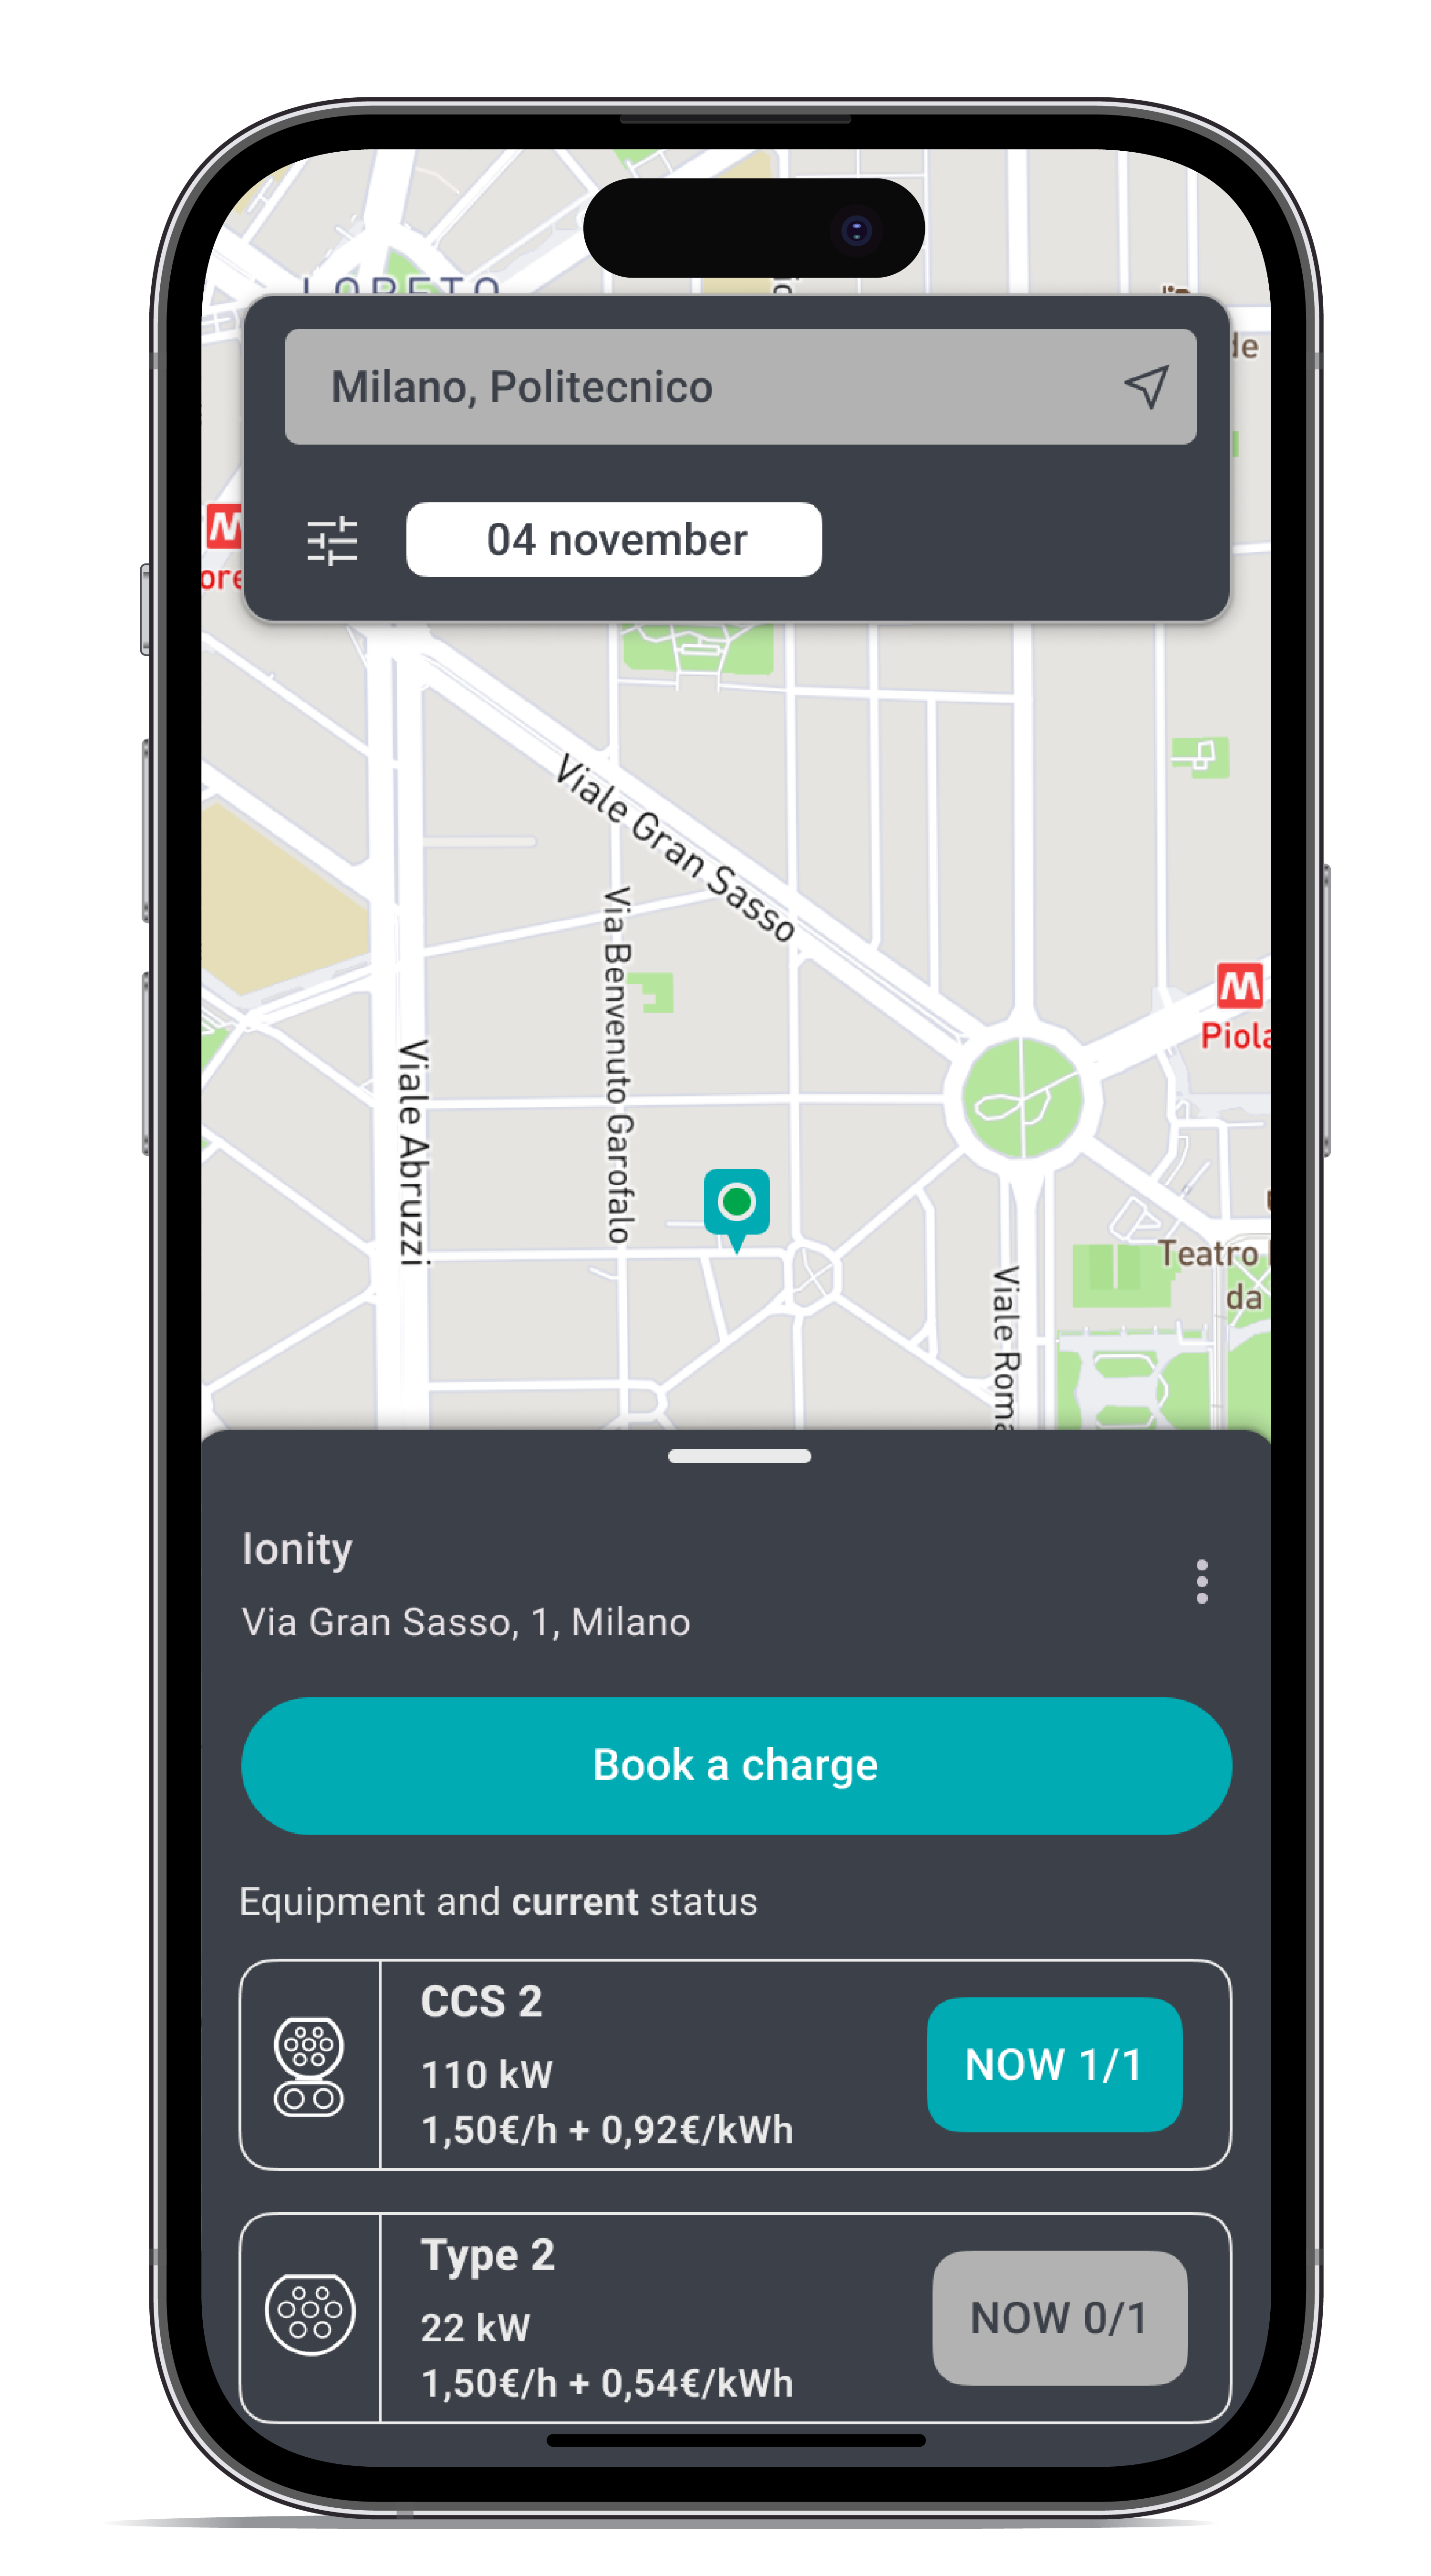
\includegraphics[scale=0.1]{src/mockups/details.png}
    }
    \subfloat[Booking]{
        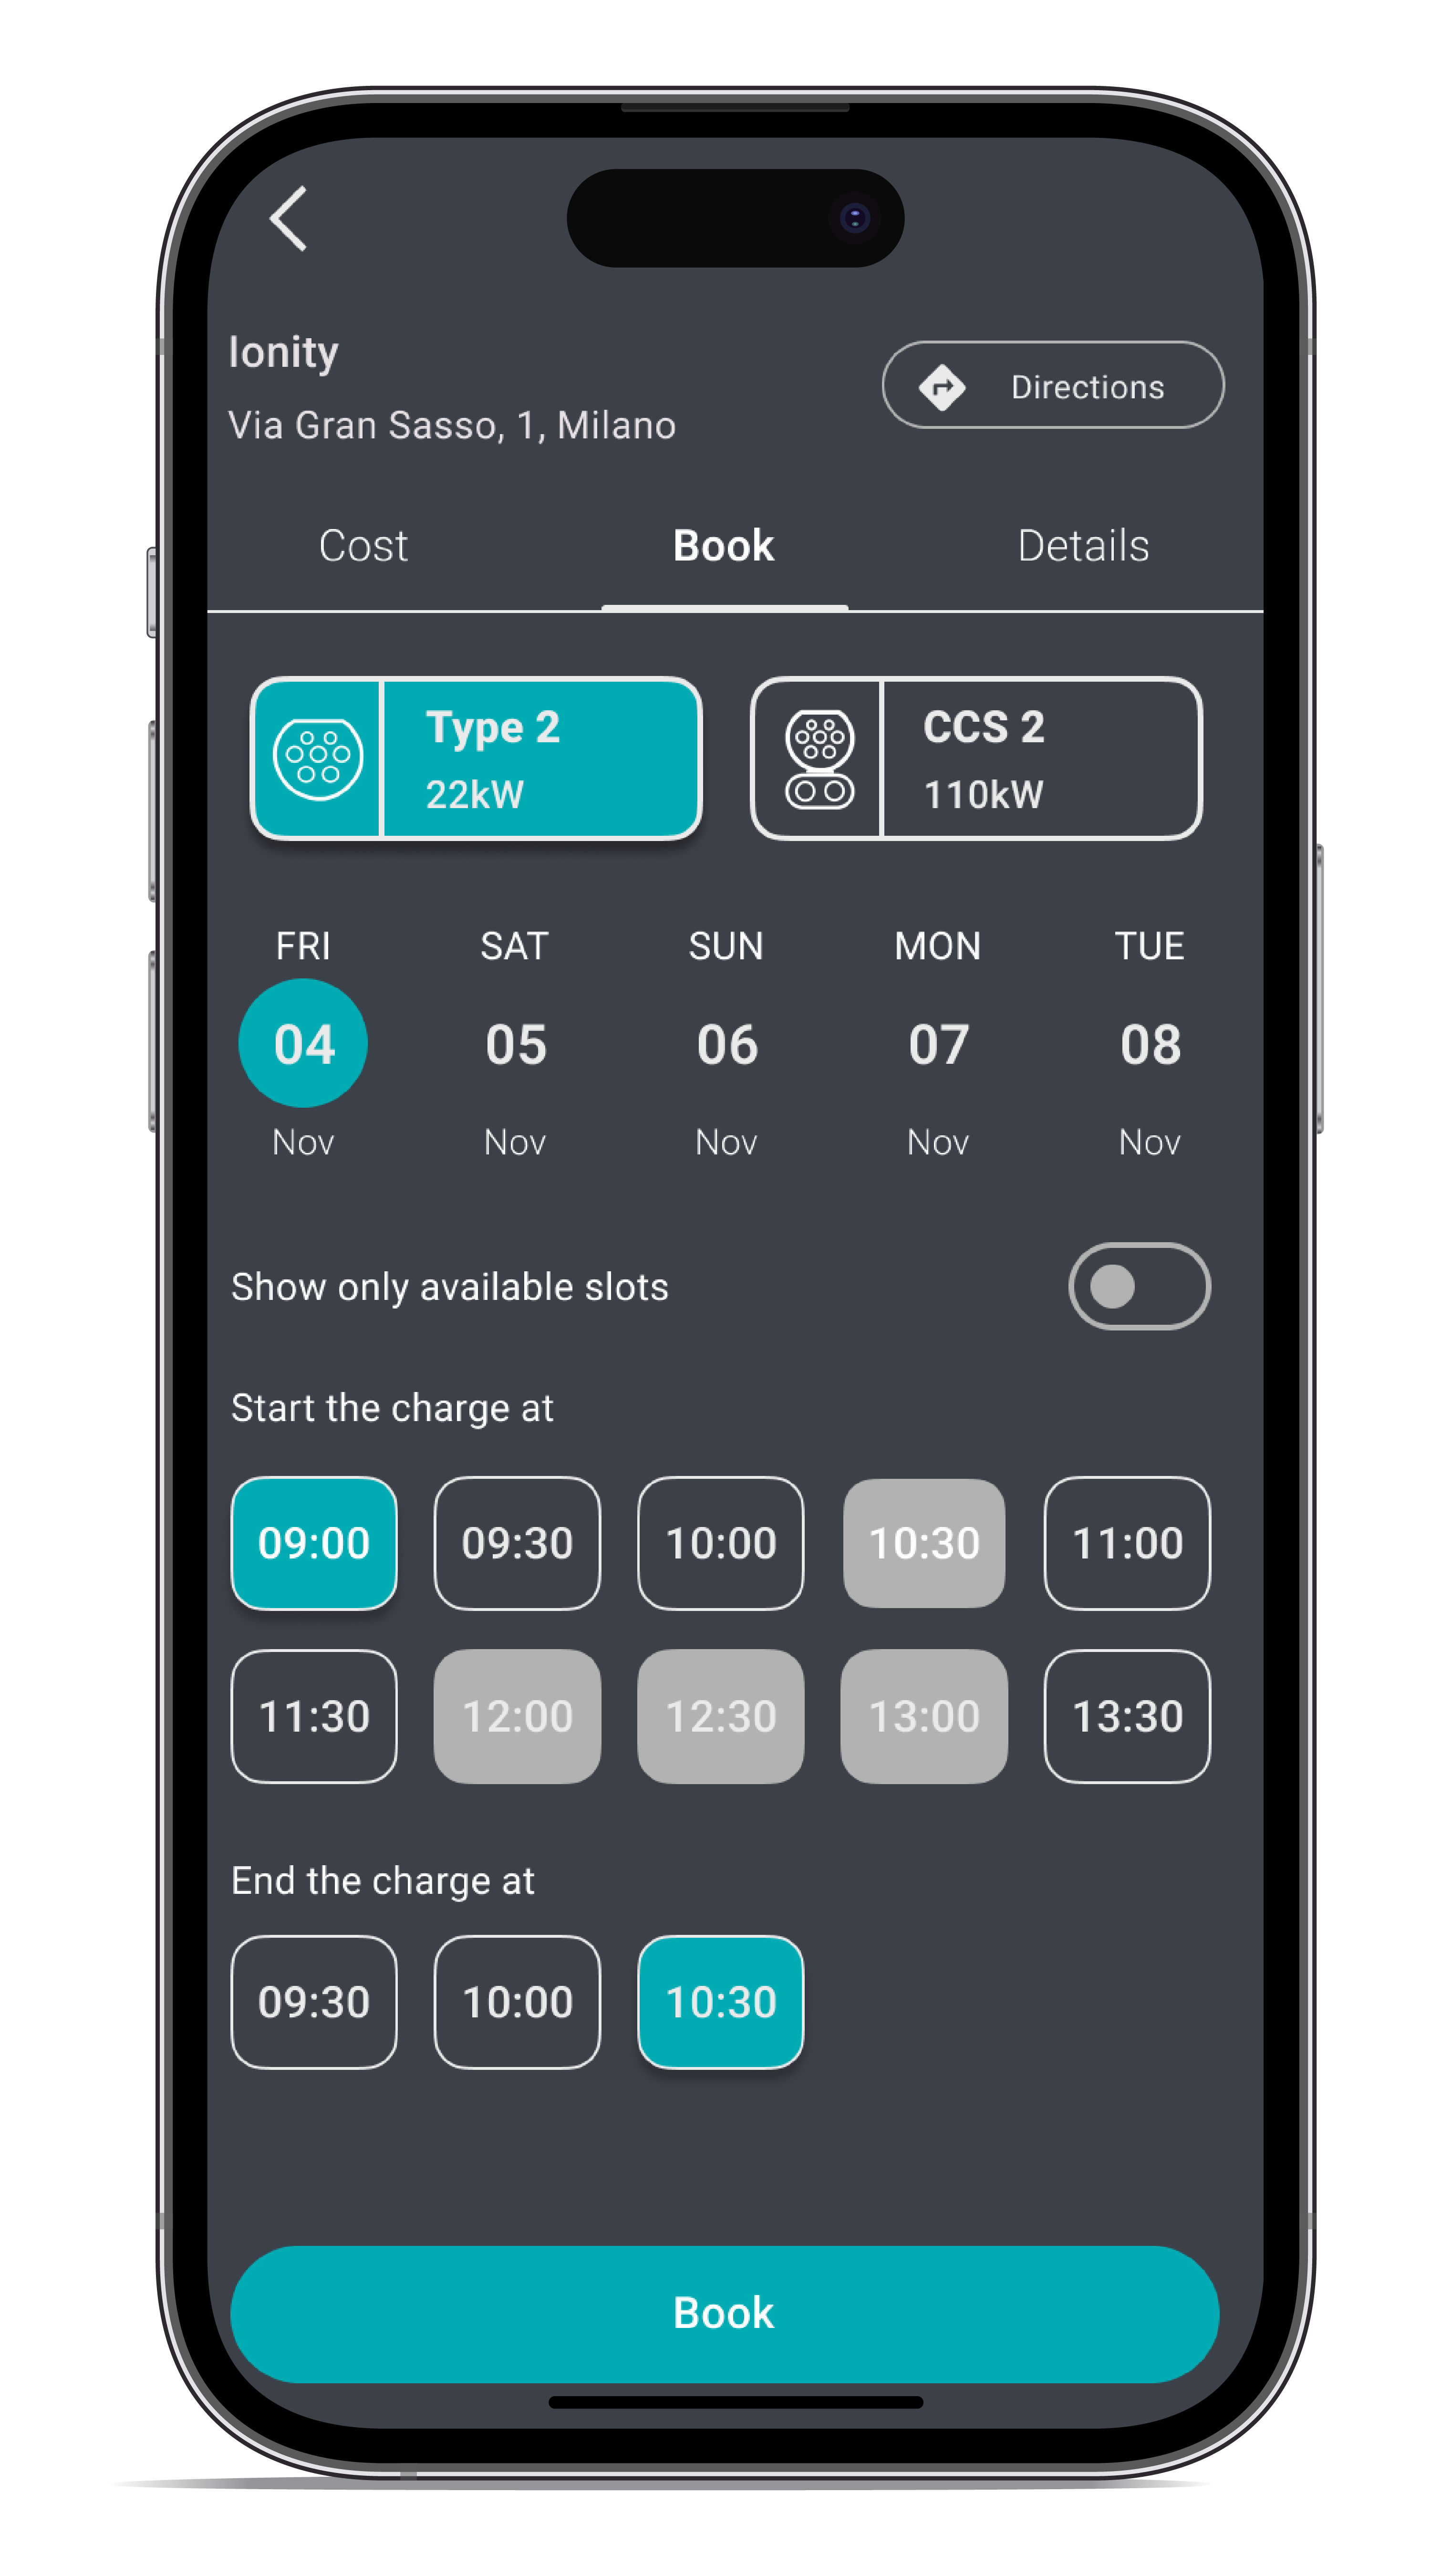
\includegraphics[scale=0.1]{src/mockups/book.png}
    }
    \subfloat[Cost detail]{
        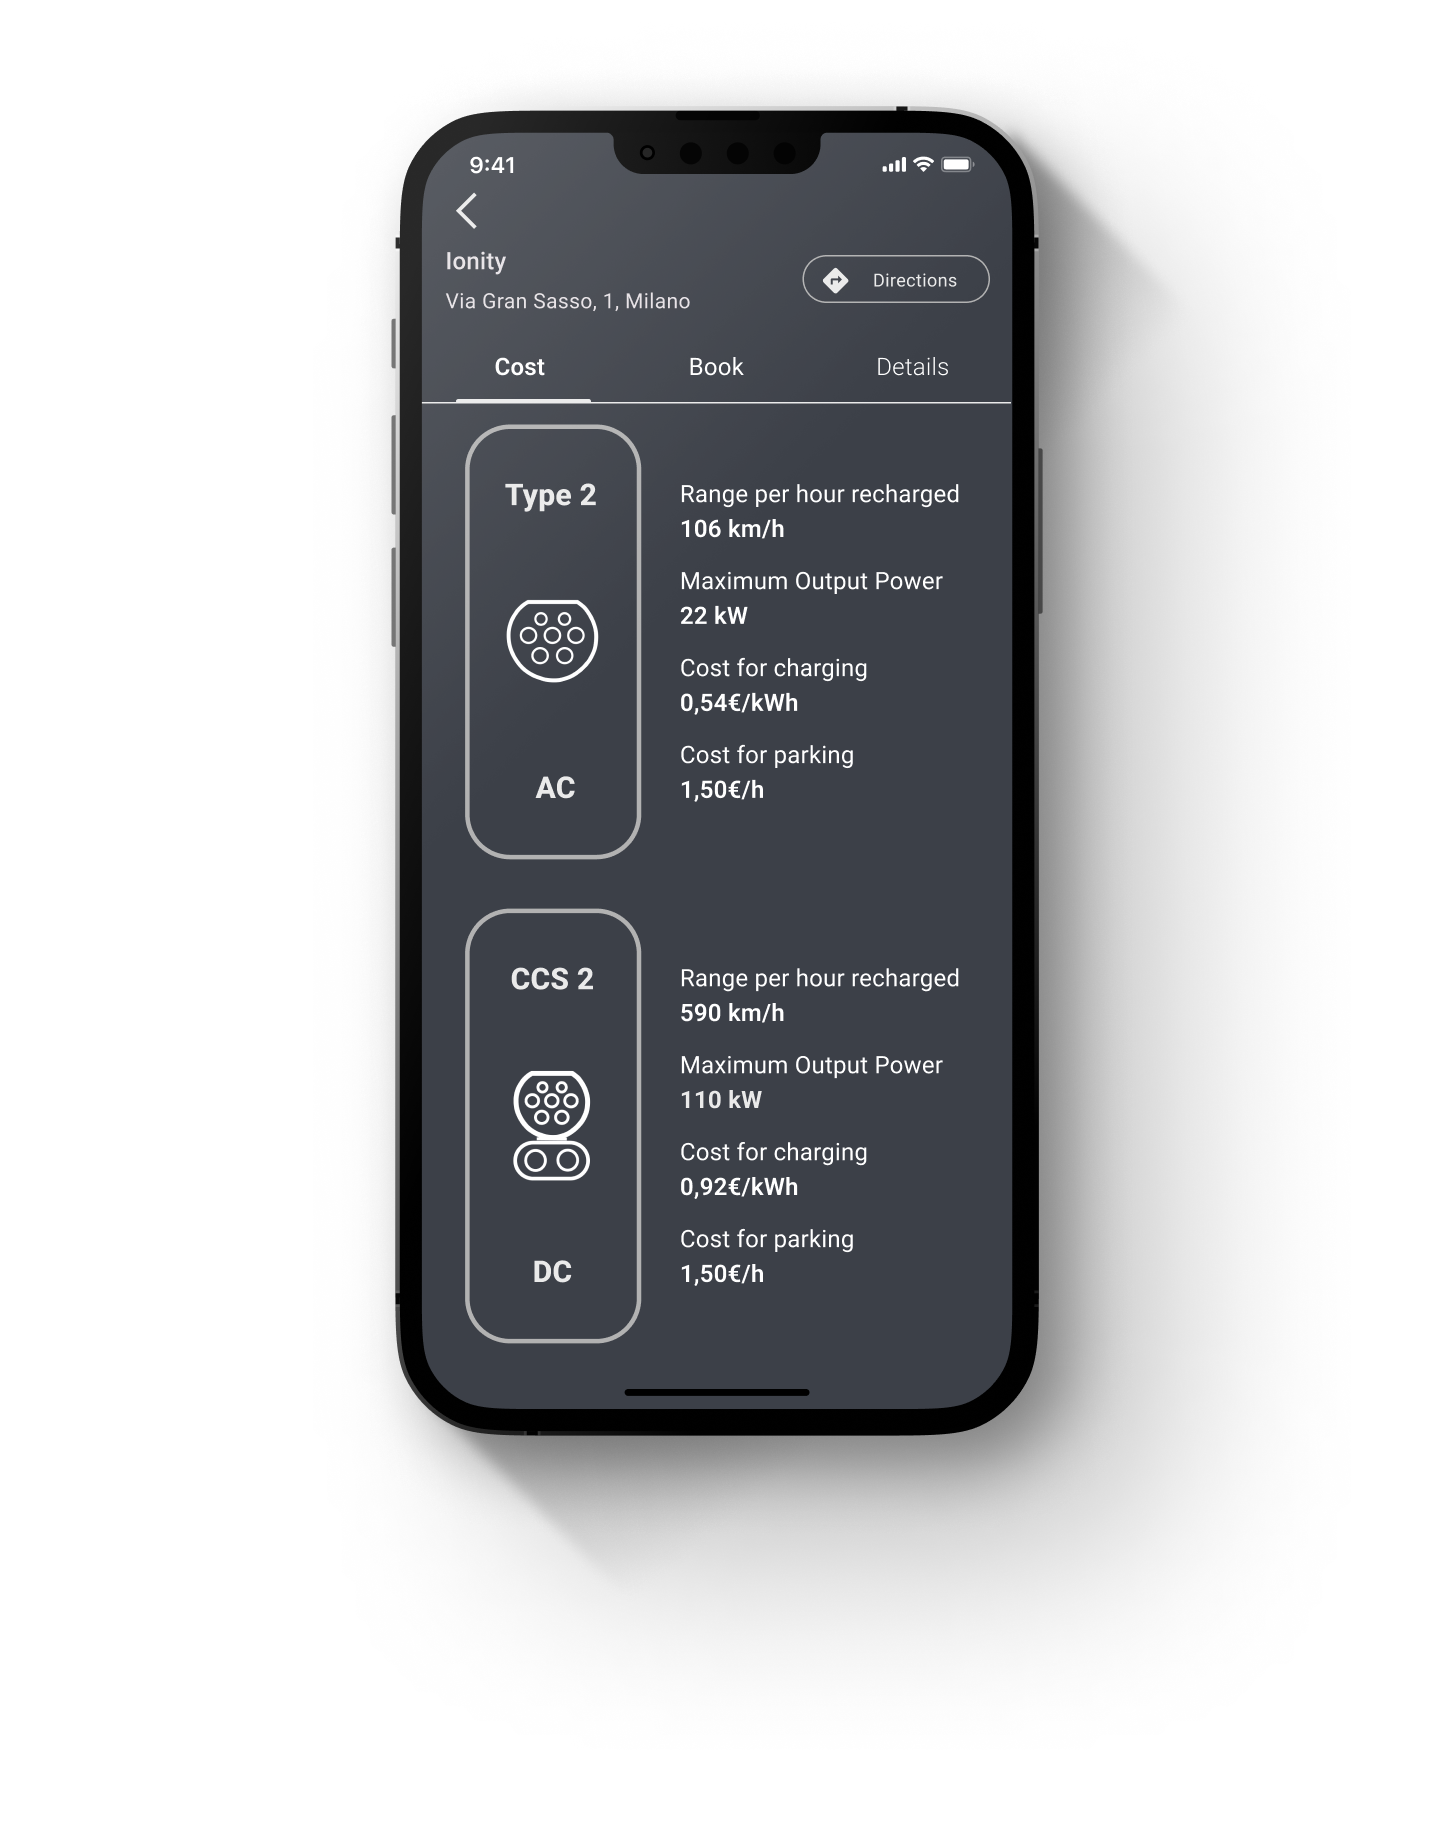
\includegraphics[scale=0.1]{src/mockups/book_cost.png}
    }
    \newline
    % following mockups
\end{figure}


\subsubsection{Hardware Interfaces}
To use the system, both EV drivers and CPOs must use a mobile device or a personal computer.
Due to the outdoor expected use of the system, a smartphone will be more suitable device 
for a EV driver, instead for a CPO is suggested to use the system from a personal computer.


\subsubsection{Software Interfaces}
The system should integrate:
\begin{itemize}
    \item a map service that provide driving direction
    and an estimation of the time required to arrive to the selected charging point 
    given a starting position (including the current EV driver position).
    \item geolocalization through GPS will be used to show the current EV driver 
    position.
    \item notifications will be sent to update in real time the EV driver 
    that the charging shift will begin shortly
    \item an SMS with a secret code will be sent both to CPO and EV driver
    upon login in order to verify their identity through a third party service.          
\end{itemize} 

\subsubsection{Communication Interfaces}
The system requires a stable internet connection to work properly.
The backend of the system will expose a unified REST compliant API to communicate
with all clients (both CPOs and EV drivers) using HTTPS and TCP/IP. 
 

\subsection{Use cases}

\begin{figure}[H]
    \centering
    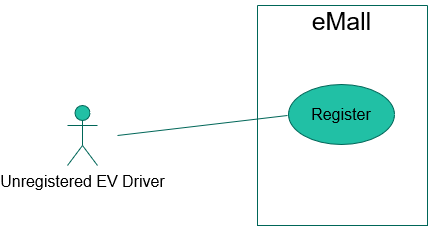
\includegraphics[scale=0.6]{src/use_case_diagram/driver_registration.png}
\end{figure}

\begin{figure}[H]
    \centering
    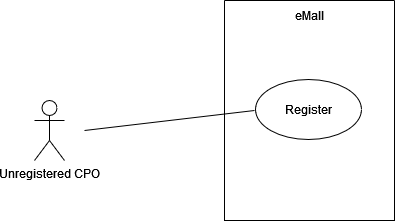
\includegraphics[scale=0.6]{src/use_case_diagram/cpo_registration.png}
\end{figure}

\begin{figure}[H]
    \centering
    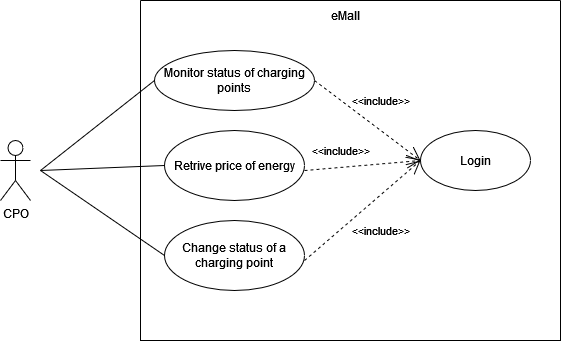
\includegraphics[scale=0.5]{src/use_case_diagram/cpo.png}
\end{figure}

\begin{figure}[H]
    \centering
    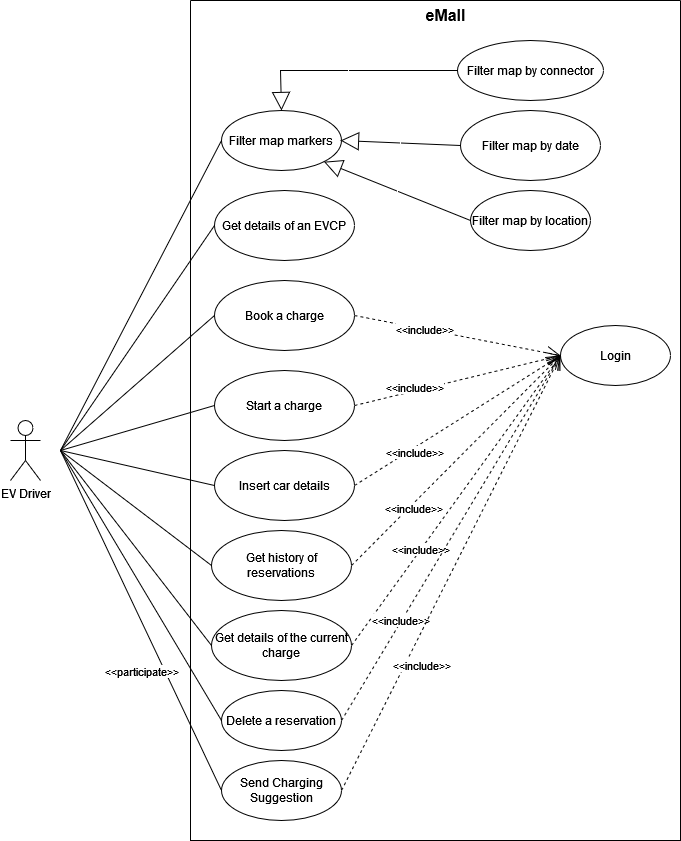
\includegraphics[scale=0.6]{src/use_case_diagram/driver.png}
\end{figure}

\usecase
{EV driver registration}
{EV driver}
{EV driver clicks 'Sign Up' in the application homepage}
{
    \begin{enumerate}
        \item The system sends user the registration form
        \item Driver enters name, surname, birth date, telephone number and password. Then submits the data upon reading and accepting the Privacy Policy and the Terms of Service
        \item The system sends a SMS to driver through an API containing a secret code
        \item The driver submits the received verification code
        \item The system verifies the code and displays a success message
    \end{enumerate}
}
{A new EV driver account is created}
{
    \begin{itemize}
        \item A required registration field is missing when the form is submitted
        \item A wrong verification code is submitted
        \item The timeout of verification expires
    \end{itemize}
}
{
    All the exception are treated the same: the system will notify user with a human-readable message and the user is redirected to the homepage
}

\usecase
{CPO registration} % name
{CPO} % actor
{CPO clicks 'Sign Up' in the business dedicated application homepage} % entry condition
{ % event flow
    \begin{enumerate}
        \item The system sends operator the registration form
        \item Operator enters company name, VAT, IBAN, and password. Then submits the data upon reading and accepting the Privacy Policy and the Terms of Service
        \item The system processes the provided information and display a success message
    \end{enumerate}
}
{A new operator account is created} % exit condition
{ % exceptions
    \begin{itemize}
        \item A required registration field is missing when the form is submitted
        \item The operator is not associated to the given VAT
        \item Loss of internet connection
        \item The actor cancels the operation

    \end{itemize}
}
{ % notes
    All the exception are treated the same: the system will notify operator with a human-readable message and the operator is redirected to the homepage
}

\usecase
{Check energy in batteries} % name
{CPO} % actor
{Authenticated CPO is in "Monitor status of EVCP" tab} % entry condition
{ % event flow
    \begin{enumerate}
        \item The operator choose a specific EVCP and clicks 'check energy in batteries'
        \item The system shows the battery status of the selected EVCP, if any
    \end{enumerate}
}
{The 'Check energy in batteries' chart is shown} % exit condition
{ % exceptions
    \begin{itemize}
        \item Loss of internet connection
        \item The actor cancels the operation
    \end{itemize}
}
{ % notes
    ...
}

\usecase
{Monitor specific charging process} % name
{CPO} % actor
{Authenticated CPO is in "Monitor status of CP" tab} % entry condition
{ % event flow
    \begin{enumerate}
        \item The operator choose a specific EVCP and clicks "monitor specific charging process"
        \item The system shows a list of active charging process and ask operator to choose one
        \item The operator choose a specific active charging process from the list
        \item The system shows the details of the chosen charging process
    \end{enumerate}
}
{The details of the specific charging process are displayed} % exit condition
{ % exceptions
    \begin{itemize}
        \item Loss of internet connection
        \item The actor cancels the operation
    \end{itemize}
}
{ % notes
...
}

\usecase
{Monitor aggregate charging process} % name
{CPO} % actor
{Authenticated CPO is in "Monitor status of CP" tab} % entry condition
{ % event flow
    \begin{enumerate}
        \item The operator choose a specific EVCP and clicks "monitor aggregate charging process"
        \item The system shows a chart with a detailed view of aggregate charging processes
    \end{enumerate}
}
{The aggregate charging process details charts are displayed} % exit condition
{ % exceptions
    \begin{itemize}
        \item Loss of internet connection
        \item The actor cancels the operation
    \end{itemize}
}
{ % notes
...
}

\usecase
{View historical reservations} % name
{CPO} % actor
{Authenticated CPO is in "View reservations" tab} % entry condition
{ % event flow
    \begin{enumerate}
        \item The operator choose a specific EVCP, choose "historical reservation" tab, and sets a specific time frame
        \item The system shows the reservation details of the chosen EVCP during the chosen time frame
    \end{enumerate}
}
{The details of the historical reservations are displayed} % exit condition
{ % exceptions
    \begin{itemize}
        \item Loss of internet connection
        \item The actor cancels the operation
    \end{itemize}
}
{ % notes
...
}

\usecase
{View active reservations} % name
{CPO} % actor
{Authenticated CPO is in "View reservations" tab} % entry condition
{ % event flow
    \begin{enumerate}
        \item The operator choose a specific EVCP, choose "active reservation" tab
        \item The system shows a list of active reservation for the chosen EVCP
    \end{enumerate}
}
{The details of the active reservations are displayed} % exit condition
{ % exceptions
    \begin{itemize}
        \item Loss of internet connection
        \item The actor cancels the operation
    \end{itemize}
}
{ % notes
...
}

\usecase
{Choose DSO} % name
{CPO} % actor
{Authenticated CPO is in "Manage CPs" tab} % entry condition
{ % event flow
    \begin{enumerate}
        \item The operator choose a specific EVCP, choose "Choose DSO" tab
        \item The system provides a list of available DSOs
        \item The operator select one DSO among the available ones and submit their choice to the system
        \item The system processes the provided information and display a success message 
    \end{enumerate}
}
{The choice of DSO is completed} % exit condition
{ % exceptions
    \begin{itemize}
        \item Loss of internet connection
        \item The actor cancels the operation
    \end{itemize}
}
{ % notes
...
}

\usecase
{Choose energy mix} % name
{CPO} % actor
{Authenticated CPO is in "Manage CPs" tab} % entry condition
{ % event flow
    \begin{enumerate}
        \item The operator choose a specific EVCP, choose "Choose energy mix" tab
        \item The system provides a list of available sources of energy (station battery, DSO, or a mix)  
        \item The operator select one source of energy among the available ones and submit their choice to the system
        \item The system shows a list of active reservation for the chosen EVCP
    \end{enumerate}
}
{The choice of a CP energy mix is completed} % exit condition
{ % exceptions
    \begin{itemize}
        \item Loss of internet connection
        \item The actor cancels the operation
    \end{itemize}
}
{ % notes
...
}

\usecase
{Retrieve price of energy} % name
{CPO} % actor
{Authenticated CPO is in "Manage CPs" tab} % entry condition
{ % event flow
    \begin{enumerate}
        \item The operator choose a specific EVCP, choose "Retrieve price of energy" tab
        \item The system provides a list of prices of sources of energy from different DSOs  
    \end{enumerate}
}
{The details of price energy are displayed} % exit condition
{ % exceptions
    \begin{itemize}
        \item Loss of internet connection
        \item The actor cancels the operation
    \end{itemize}
}
{ % notes
...
}

\usecase
{Change Status of a CP} % name
{CPO} % actor
{Authenticated CPO is in "Manage CPs" tab} % entry condition
{ % event flow
    \begin{enumerate}
        \item The operator choose a specific EVCP, choose "Change Status of a CP" tab 
        \item The system provides a page on which the operator can set a specific time frame in which the operator wants to change the status of CP  
        \item The operator set a specific time frame
        \item The system processes the provided information and display a success message 
    \end{enumerate}
}
{The status of a CP is displayed} % exit condition
{ % exceptions
    \begin{itemize}
        \item Loss of internet connection
        \item The actor cancels the operation
    \end{itemize}
}
{ % notes
...
}



\subsection{Functional Requirements}


\subsubsection{CPO Functional Requirements}
\begin{table}[H]
    \begin{tabularx}{\textwidth}{cX}
        \toprule
        \textbf{R1}  & The system must allow unregistered operator to register an account and its EVSEs                                                  \\
        \textbf{R2}  & The system must allow making a special offer                                                                                      \\
        \textbf{R3}  & The system must allow monitoring the charging process to infer when the battery is full                                           \\
        \textbf{R4}  & The system must allow retrieving details on the amount of energy available in its EVSEs batteries                                 \\
        \textbf{R5}  & The system must allow retrieving details on the number of vehicle being charged and for each vehicle the amount of absorbed power \\
        \textbf{R6}  & The system must allow retrieving details on the charge time left for each connected vehicle                                       \\
        \textbf{R7}  & The system must allow retrieving details on active and historical reservations on its EVSEs                                       \\
        \textbf{R8}  & The system must allow acquiring information from the DSOs about the current price of energy                                       \\
        \textbf{R9}  & The system must allow deciding from which DSO to acquire energy from                                                              \\
        \textbf{R10} & The system must dynamically decide where to get energy for charging (electrical grid, battery or a mixture)                       \\
        \textbf{R11} & The system must allow add, modify and delete a CP                      \\
        \bottomrule
    \end{tabularx}
\end{table}
\subsubsection{eMSP Functional Requirements}
\begin{table}[H]
    \begin{tabularx}{\textwidth}{cX}
        \toprule
        \textbf{R11} & The system must allow unregistered users to register an account                                                     \\
        \textbf{R12} & The system must allow registered users to login                                                                     \\
        \textbf{R13} & The system must allow authenticated users to personalize their experience by providing information of their EV      \\
        \textbf{R14} & The system must allow users to search for EVSEs in the map                                                          \\
        \textbf{R15} & The system must show to the users EVSEs nearby their current position                                               \\
        \textbf{R16} & The system must allow retrieving details on a given EVSE regarding connector types supported and cost of the charge \\
        \textbf{R17} & The system must allow booking of an EVSE for a certain time interval                                                \\
        \textbf{R18} & The system must allow booking of an EVSE if and only if it is free for the specified time interval                  \\
        \textbf{R19} & The system must notify users when the charging shift is about to start                                              \\
        \textbf{R20} & The system must allow authenticated users to start the charge                                                       \\
        \textbf{R21} & The system must suggest users when to charge based on daily schedule, special offers and availability               \\
        \textbf{R22} & The system must allow authenticated users to monitor the charging status                                            \\
        \textbf{R23} & The system must notify authenticated users when the charging process is completed                                   \\
        \textbf{R24} & The system must allow authenticated users to pay for the charge                                                     \\
        \textbf{R25} & The system must allow authenticated users to delete a reservation                                                   \\
        \textbf{R26} & The system must allow authenticated users to view historical reservations                                           \\ \bottomrule
    \end{tabularx}
\end{table}

\subsubsection{Mapping on requirement}
\begin{table}[H]
    \begin{tabularx}{\textwidth}{XXX}
        \toprule
        \textbf{Goal} & \textbf{Requirements} & \textbf{Assumptions} \\ \midrule
        G1            & R1,R2,R3              & D1,D2,D3             \\
        G2            & esempio               & esempio              \\
        G3            & esempio               & esempio              \\ \bottomrule
    \end{tabularx}
\end{table}

\subsection{Performance Requirements}
The requirements of the system are not critical, so these performance requirements
are focus on guarantee the best of possible experience to both EV drivers and CPOs.
To do that, the system should provide:
• a scalable, reactive and load-balancing backend
• the visualization of the map in 5 seconds, or less;
• the list of active and historical reservations in less than 5 seconds;
• the booking confirmation in 7 seconds, or less;
• the loading of the available time slots for a specific charging point in less than 5 seconds;
• push app notification with a delay that is imperceptible to the user.
• Notice that a good internet connection is assumed in the previous estimations.

\subsection{Design Constraints}


\subsubsection{Standards compliance}
Specifications described in this document must be respected by the system.
Source code of the application must be commented on and documented adequately.
The system should respect the line guides described by the European GDPR.

\subsubsection{Hardware limitations}
The system requires any device and a stable internet connection.

\subsection{Software System Attributes}

\subsubsection{Availability and Reliability}
The system should offer its functionalities with an availability
equal to 99.5, or more. In other words, the system must be inaccessible 
for less than two days every year. To achieve this goal, the system should
provide a high redundancy for the most critical components.
Furthermore, in order to guarantee better reliability performances, all 
the scheduled maintenance intervents on the system should be done during
the night.

\subsubsection{Security}
The connection between the application and the server must be safe.
System use the TLS (Transport Layer Security) protocol.
To do that for this purpose, it is needed an SSL/TSL certificate. 
Moreover, all passwords must be encrypted

\subsubsection{Maintainability}
Source code and correlated documentation must be commented and kept updated.
Modularity, low coupling and high cohesion between components must be a focus during the 
designing and developing phases.

\subsubsection{Portability}
The system is a web application so it will be supported by any device with
a modern browser.